\documentclass[epsfig,a4paper,11pt,titlepage,twoside,openany]{book}
\usepackage{epsfig}
\usepackage{plain}
\usepackage{setspace}
\usepackage[paperheight=29.7cm,paperwidth=21cm,outer=1.5cm,inner=2.5cm,top=2cm,bottom=2cm]{geometry} % per definizione layout
\usepackage[explicit]{titlesec}
\usepackage{amsmath}
\usepackage{amsthm}
\usepackage{amssymb}
\usepackage[hidelinks]{hyperref}
\usepackage{algorithm}
\usepackage{algpseudocode}
\usepackage{marvosym}

\singlespacing{}

%definizioni e teoremi
\theoremstyle{definition}
\newtheorem{definizione}{Definizione}[chapter]
\newtheorem{problema}[definizione]{Problema}

\theoremstyle{plain}
\newtheorem{teorema}[definizione]{Teorema}
\newtheorem{lemma}[definizione]{Lemma}
\newtheorem{proposizione}[definizione]{Proposizione}
\newtheorem{corollario}[definizione]{Corollario}

\usepackage[italian]{babel}

\begin{document}
\pagenumbering{gobble}
\pagestyle{plain}

\thispagestyle{empty}

\begin{center}
  \begin{figure}[h!]
    \centerline{
\psfig{file=marchio_unitrento_colore_it_202002.eps,width=0.6\textwidth}}
  \end{figure}

  \vspace{2 cm} 

  \LARGE{Dipartimento di Matematica\\}

  \vspace{1 cm} 
  \Large{Corso di Laurea in Matematica\\}

  \vspace{2 cm} 
  \Large\textsc{Elaborato finale\\} 
  \vspace{1 cm} 
  \Huge\textsc{Grafi planari\\}
  \Large{\textit{Algoritmo di Boyer per l'immersione planare e l'isolamento di un sottografo di Kuratowski}}


  \vspace{2 cm} 
  \begin{tabular*}{\textwidth}{ c @{\extracolsep{\fill}} c }
  \Large{Supervisore} & \Large{Laureando}\\
  \Large{Alberto Montresor}& \Large{Martino Papa}\\
  \end{tabular*}

  \vspace{2 cm} 

  \Large{Anno accademico 2023/2024}
  
\end{center}



\clearpage

\thispagestyle{empty}

\begin{center}
  {\bf \Huge Ringraziamenti}
\end{center}

\vspace{4cm}


\emph{
  grazie
}

\clearpage{}
\pagestyle{plain}
\mainmatter{}

\tableofcontents
\clearpage


\begingroup
% \renewcommand{\cleardoublepage}{} 
% \renewcommand{\clearpage}{} 

% \titlespacing*{\chapter}{0pt}{0.59in}{0.02in}
% \titlespacing*{\section}{0pt}{0.20in}{0.02in}
% \titlespacing*{\subsection}{0pt}{0.10in}{0.02in}

\chapter*{Sommario} % senza numerazione
\label{sommario}

\addcontentsline{toc}{chapter}{Sommario} % da aggiungere comunque all'indice

Lorem ipsum dolor sit amet, consectetur adipiscing elit. Donec sed nunc orci. Aliquam nec nisl vitae sapien pulvinar dictum quis non urna. Suspendisse at dui a erat aliquam vestibulum. Quisque ultrices pellentesque pellentesque. Pellentesque egestas quam sed blandit tempus. Sed congue nec risus posuere euismod. Maecenas ut lacus id mauris sagittis egestas a eu dui. Class aptent taciti sociosqu ad litora torquent per conubia nostra, per inceptos himenaeos. Pellentesque at ultrices tellus. Ut eu purus eget sem iaculis ultricies sed non lorem. Curabitur gravida dui eget ex vestibulum venenatis. Phasellus gravida tellus velit, non eleifend justo lobortis eget.


  Sommario è un breve riassunto del lavoro svolto dove si descrive l'obiettivo, l'oggetto della tesi, le 
metodologie e le tecniche usate, i dati elaborati e la spiegazione delle conclusioni alle quali siete arrivati.  

Il sommario dell'elaborato consiste al massimo di 3 pagine e deve contenere le seguenti informazioni:
\begin{itemize}
  \item contesto e motivazioni 
  \item breve riassunto del problema affrontato
  \item tecniche utilizzate e/o sviluppate
  \item risultati raggiunti, sottolineando il contributo personale del laureando/a
\end{itemize}





\chapter{Introduzione}
\chapter{Fondamenti teorici}

Nel 1736 Leonhard Euler (1707~-~1783) decise di cimentarsi nel risolvere il problema dei sette ponti di Königsberg, nella sua pubblicazione “\textit{Solutio problematis ad geometriam situs pertinentis}\cite{ponti}” Eulero dimostò la non esistenza della soluzione di tale problema. Per farlo inventò quella che ad oggi chiamiamo teoria dei grafi.
\begin{definizione}[Grafo]
    Un grafo è una coppia \(G=(V,E)\) dove:
    \begin{itemize}
        \item \(V\) è un insieme di vertici (\textbf{vertex});
        \item \(E\) è un insieme di coppie di nodi \((u,v),\;u,v\in V\) dette archi o lati (\textbf{edge}); se un grafo è orientato avremmo che le coppie \(<u,v>\in E\) saranno ordinate.
    \end{itemize}
\end{definizione}
\noindent In questo documento assumeremo sempre \(G\) non orientato. 
\begin{definizione}[Grafo planare]\label{grafo-planare}
    Un grafo \(G\) si dice planare se può essere rappresentato nel piano evitando che gli archi si intersechino (se non negli endpoint).
\end{definizione}
Uno dei quesiti più interessanti riguardante la teoria dei grafi è riuscire stabilire se un determinato grafo \(G\) sia planare o meno. Nonostante la definizione di questo problema sia molto semplice, la soluzione non è affato banale. Lo studio di algoritmi efficienti per il “\textit{planarity testing}”  è stato infatti affrontato da molteplici matematici nel corso del 1900 e dei primi anni 2000.\\
Il primo algoritmo in grado di risolvere tale problema in tempo lineare fu “\textit{l'algoritmo di Hopcroft e Tarjan}\cite{Hopcroft}” pubblicato nel 1974. Esso si limitava però a fornire in output un valore booleano senza “disegnare” una reale immersione planare di \(G\).
\begin{definizione}[Immersione planare]
    Dato un grafo \(G\), definiamo \(\psi : (V,E) \to \mathbb{R}^2\) la funzione che mappa i vertici di \(G\) nel piano e gli archi di \(G\) in curve continue che si intersecano solamente negli endpoint. Allora \(G^\psi \doteq \psi(G)\) è chiamata immersione planare di \(G\).
\end{definizione}
Solamente 30 anni dopo, grazie alla pubblicazione John M. Boyer “\textit{Simplified \(O(n)\) Planarity by Edge Addition}\cite{main_article}”, è stato scoperto il primo algoritmo lineare in grado di resituire, se \(G\) planare, una sua immersione mentre, se \(G\) non planare, un sottografo di Kuratowski contenuto in esso. Dimostreremo infatti nel teorema \(\ref{Kuratowski}\) che un grafo \(G\) è non planare se e solo se contiene un sottografo di Kuratowski.
\begin{definizione}[Grafo di Kuratowski]\label{kuratowskisottografo}
    Definiamo \(K_{3,3}\) e \(K_5\) grafi di Kuratowski.
\end{definizione}
\section{Formulazione di ipotesi non restrittive}
Abbiamo stabilito che determinare la planarità di un grafo non sia un quesito facile. Tuttavia ci sono alcuni risultati matematici in grado di fornire risposte immediate per alcuni casi paritcolari. Questo ci permetterà di escludere a priori la possibilità che tali grafi siano planari.
\begin{teorema}\label{eulero-generica}
    Sia \(G\) un grafo planare avente \(k\) componenti connesse. Sia \(G^\varphi\) una immersione di \(G\) nel piano, allora
    \begin{equation}
        \chi(G)=V+f-\epsilon = k+1
    \end{equation}
    dove \(V\) è il numero di vertici (\(k_0\)), \(\epsilon\) il numero di archi (\(k_1\)), \(f\) il numero di facce (\(k_2\)), \(\chi(G)\) la caratteristica di eulero \(\ref{caratteristica-eulero}\).
    \begin{proof}
        Procediamo per induzione sul numero di archi \( \epsilon \): \smallskip \\
        \underline{caso base \(\epsilon=0\)}, \(V=k\) vertici, \(f=1\) quindi è soddisfatta \(V-\epsilon+f = k+1\)\smallskip \\
        \underline{passo induttivo \(\epsilon \to \epsilon + 1\)}, aggiungiamo un arco al grafo
        \begin{enumerate}
            \item \textit{il nuovo arco è un loop}, in questo caso \(V \to V\), \(\epsilon \to \epsilon +1\), \(f \to f+1\), \(k \to k\) e quindi
                  \begin{equation}
                      V-(\epsilon+1)+(f+1)=V-\epsilon+f=k+1
                  \end{equation}
            \item \textit{il nuovo arco è tra due vertici appartenenti alla stessa componente connessa}, anche in questo caso \(V \to V\), \(\epsilon \to \epsilon +1\), \(f \to f+1\), \(k \to k\) e quindi
                  \begin{equation}
                      V-(\epsilon+1)+(f+1)=V-\epsilon+f=k+1
                  \end{equation}
            \item \textit{il nuovo arco connette due componenti che erano sconnesse}, in questo caso \(V \to V\), \(\epsilon \to \epsilon +1\), \(f \to f\), \(k \to k-1\) e quindi
                  \begin{equation}
                      V-(\epsilon +1)+f = (k-1) + 1 = k'+1
                  \end{equation}
                  dove \(k'=k-1\) è il numero di componenti connesse dopo l'aggiunta dell'arco.
        \end{enumerate}
    \end{proof}
\end{teorema}
\begin{corollario}[Formula di Eulero]\label{formulaeulero}
    Sia \(G\) un grafo planare connesso, allora
    \begin{equation}
        \chi(G)=V+f-\epsilon = 2
    \end{equation}
    \begin{proof}
        Direttamente dal teorema \(\ref{eulero-generica}\) con \(k=1\).
    \end{proof}
\end{corollario}
Notiamo che questi due risultati non forniscono immediate risposte riguardo alla planarità di un determinato grafo \(G\). Per conoscerne il numero di facce è infatti necessario ottenere una immersione planare di esso. Tuttavia il corollario \(\ref{formulaeulero}\) sarà fondamentale in alcune dimostrazioni che vedremo successivamente.
\begin{lemma}\label{gradifacce}
    Sia \(G\) un grafo planare, \(G^\psi\) una sua immersione nel piano, \(F_1, \dots, F_f\) le facce di \(G^\psi\) allora
    \begin{equation}
        \sum_{i=1}^f \deg(F_i) = 2\epsilon
    \end{equation}
    \begin{proof}
        Segue direttamente dal fatto che ogni arco \((u,v)\) è incedente esattamente su due facce di \(G^\psi\).
    \end{proof}
\end{lemma}
Combinando i risultati del lemma \(\ref{gradifacce}\) e del corollario \(\ref{formulaeulero}\), otteniamo questa importante proposizione che ci permette di stabilire a priori se determinati grafi siano non planari.
\begin{proposizione}\label{criterioNonPlan}
    Sia \(G\) planare, \(\epsilon\) il numero di archi, \(V\) il numero di vertici. Vale allora
    \begin{equation}
        \epsilon \leq 3V - 3
    \end{equation}
    Inoltre se supponiamo \(V \geq 3\) vale
    \begin{equation}
        \epsilon \leq 3V - 6
    \end{equation}
    \begin{proof}
        Sia \(V<3\). In questo caso il lemma è una diretta conseguenza della formula di Eulero (Teorema {\ref{formulaeulero}}). \\
        Sia \(V\geq 3\). \(G\) planare \(\Rightarrow\) ogni faccia ha almeno 3 lati ovvero \(\deg(F_i) \geq 3\; \forall i\). Per il lemma {\ref{gradifacce}} vale quindi
        \begin{equation}
            2\epsilon = \sum_{i=1}^f \deg(F_i) \geq \sum_{i=1}^f 3 = 3f
        \end{equation}
        Per la formula di eulero segue inoltre \(V+f-\epsilon = 2\) da cui abbiamo, moltiplicando per 3 e riarrangiando i termini
        \begin{equation}
            3\epsilon = 3V + 3f - 6
        \end{equation}
        applicando ora \(3f\leq 2 \epsilon\) otteniamo la tesi.
    \end{proof}
\end{proposizione}
Vediamo ora un altra serie di risultati che ci permetteranno di formulare ulteriori ipotesi non restrittive sul grafo analizzato.
\begin{proposizione}
    Ogni suddivisione di un grafo non planare è non planare, questo implica anche che i vertici di grado 2 non influenzano la planarità del grafo.
    \begin{proof}
        Sia \(G\) grafo non planare, \(a,b\) due archi che si intersecano nell'immersione \(G^\psi\), è evidente che suddividere \(a\) o \(b\) non andrebbe ad influire sulla non planarità del grafo.
    \end{proof}
\end{proposizione}
\begin{proposizione}\label{Blocchi}
    Un grafo separabile è planare se e solo se tutti i suoi blocchi sono planari.
    \begin{proof}
        \underline{“\(\Rightarrow\)”}: banale, è evidente che se un grafo è planare allora anche i suoi sottografi lo sono.\\
        \underline{“\(\Leftarrow\)”}: notiamo che due blocchi differenti hanno al più un elemento nell'intersezione, se così non fosse i due blocchi sarebbero 2-connessi confutando l'ipotesi di massimalità. Proseguiamo ora per induzione sul numero di blocchi \(|B|\), dove \(B={\{b_i\}}_{i \in I}\) è l'insieme dei blocchi.
        \begin{itemize}
            \item \textit{caso base}: \(G\) 2-connesso quindi \(|B|=1\), \(B=\{G\}\) e la tesi equivale a “\(G \text{ planare} \Rightarrow G \text{ planare}\)”.
            \item \textit{passo induttivo}: sia \(G\) grafo composto da \(n\) cicli. Rimuoviamo da \(G\) un blocco \(b\) che si intersechi solo con un altro blocco \(b'\) nel veritce \(v\), questo deve esistere perchè altrimenti sarebbe presente un ciclo di blocchi, essi sarebbero dunque 2-connessi e di coneseguenza non massimali \(\text{\Lightning}\); 
            potrebbe anche essere che tutti i blocchi siano sconnessi e quindi la loro intersezione sarebbe sempre vuota, tuttavia questo è un caso banale in quanto è evidente che un grafo è planare se e solo se tutte le sue componenti connesse sono planari. 
            \\ Il grafo \(G'\) risultante dalla rimozione del blocco \(b\) è per ipotesi induttiva planare, disegnamo ora le immersioni nel piano di \(b\) e \(G'\) facendo in modo che il punto di intersezione \(v\) appaia in entrambe le immersioni nella faccia esterna. Possiamo ora unire tra loro le due immersioni ottenendo che \(G=G' \cup b\) è planare.
        \end{itemize}
    \end{proof}
\end{proposizione}
\begin{lemma}
    Un grafo è planare se e solo se tutte le sue componenti conesse sono planari.
    \begin{proof}
        Caso banale dimostrato nel lemma precedente (\(\ref{Blocchi}\)).
    \end{proof}
\end{lemma}
Grazie alla proposizione \(\ref{Blocchi}\) possiamo sempre supporre \(G\) 2-connesso senza perdere generalità.
\section{Il teorema di Kuratowski}
Come accennato in precedenza gli algoritmi di planarity testing moderni non si limitano a fornire una risposta booleana per la planarità, bensì, in caso di risposta negativa, essi restituiscono in output un sottografo di Kuratowski (\(\ref{kuratowskisottografo}\)). Il nome di tali sottografi è dovuto al matematico polacco Kazimierz Kuratowski, fu lui infatti a dimostrare che la presenza di un tale sottografo è equivalente alla non planarità.
\\ Vediamo ora i risultati teorici che permettono di raggiungere tale conclusione.
\begin{lemma}\label{k5k33nonplanari}
    \(K_5\) e \(K_{3,3}\) sono grafi non planari.
    \begin{proof}
        \underline{\(K_5\)}: il grafo completo \(K_n\) ha \(\epsilon=\frac{n(n-1)}{2}\) archi. Supponendo per assurdo \(K_5\) planare dovrebbe valere la proposizione \(\ref{criterioNonPlan}\) ovvero, essendo \(V=5 \geq 3\)
        \begin{equation}
            10 = \frac{n(n-1)}{2} = \epsilon \leq 3V-6 = 9 \rightarrow \text{\Lightning}
        \end{equation}
        \underline{\(K_{3,3}\)}: Supponendo per assurdo \(K_{3,3}\) planare, sapendo \(\epsilon=3*3=9\), \(V=6\) dalla formula di eulero \(\ref{formulaeulero}\) otterremmo \(f=2-V+\epsilon=5\). \\
        Siccome \(K_{3,3}\) è bipartito, esso non contiene cicli composti da 3 archi, quindi ogni faccia ha almeno 4 lati, ovvero \(\deg(F)\geq 4 \;\forall F\) e vale \(\sum_{i=1}^{f} \deg(F_i) \geq 4*f = 20\). Applicando ora il lemma \(\ref{gradifacce}\) otteniamo l'assurdo
        \begin{equation}
            20 \leq \sum_{i=1}^{f} \deg(F_i) = 2\epsilon = 18 \rightarrow\text{\Lightning}
        \end{equation} 
    \end{proof}
    \begin{figure}[H]
        \centering
        
\includegraphics[scale=0.6]{img/k533.PNG}
        \caption{\(K_5\) e \(K_{3,3}\)}
    \end{figure} 
\end{lemma}
\begin{lemma}\label{12.3}
    Sia \(G\) un grafo qualsiasi ottenuto splittando un vertice di \(K_5\) allora \(G\) contiene un sottografo \(TK_{3,3}\).
    \begin{proof}
        Siano \(u_1, u_2\) i due vertici risultanti dallo split di un vertice di \(K_5\). Per definizione di split ambedue i vertici hanno almeno grado 3. \(u_1\) e \(u_2\) sono adiacenti e assieme sono adiacenti a tutti i rimanenti 4 vertici. Scegliendo ora una partizione dei 4 vertici \(x,y,w,z\) t.c. \(u_1\) adiacente a \(x,y\) e \(u_2\) adiacente a \(w,z\), otteniamo un sottografo \(K_{3,3}\) con bipartizione \((u_1, w, z)\) e \((u_2,x,y)\).
    \end{proof}
\end{lemma}
\begin{teorema}\label{minoreTK5}
    Se \(G\) ha un minore \(K_{3,3}\) allora contiene un sottografo \(TK_{3,3}\). Se \(G\) ha un minore \(K_5\) allora contiene un sottografo \(TK_{3,3}\) o \(TK_5\).
    \begin{proof}
        Supponiamo che \(G\) abbia un minore \(TK_{3,3}\) o \(TK_5\), se nel ottenere il minore non è stata coinvolta nessuna operazione di contrazione degli archi allora esso sarà anche un sottografo di \(G\). Altrimenti sia \(G_0,\dots, G_k\) sequenza di grafi ottenuta da \(G\), \(G_0\) sottografo di \(G\), l'arco \(e_i\) di \(G_{i-1}\) è contratto per ottenere \(G_i\) e \(G_k\) è \(K_{3,3}\) o \(K_5\).
        Se ogni \(e_i\) ha un endpoint di grado 2 possiamo invertire la contrazione suddividendo gli archi e trovando un sottografo \(TK_{3,3}\) o \(TK_5\). 
        \\ Altrimenti sia \(e_i\) l'arco con \(i\) massimo tra quelli con entrambi gli endpoint di grado almeno 3. Tutti gli archi contratti successivamente a \(G_i\) hanno un endpoint di grado 2, quindi \(G_i\) ha un sottografo \(TK_{3,3}\) o \(TK_5\). \(G_{i-1}\) può essere ottenuto splittando un vertice \(u \in G_i\), analizziamo ora i 3 casi:
        \begin{itemize}
            \item \textit{\(u\) appartiene a \(TK_5\)}: per il lemma \(\ref{12.3}\) \(G_{i-1}\) conterrà un sottografo \(TK_{3,3}\);
            \item \textit{\(u\) appartiene a \(TK_{3,3}\)}: anche \(G_{i-1}\) conterrà quindi \(TK_{3,3}\);
            \item \textit{\(u\) non appartiene a \(TK_{3,3}\) e \(TK_5\)}: in \(G_{i-1}\) sarà quindi ancora presente \(TK_{3,3}\) o \(TK_5\).
        \end{itemize}
    \end{proof}
\end{teorema}
Abbiamo ora tutti i prerequisiti necessari per dimostrare il teorema di Kuratowski.
\begin{teorema}[Teorema di Kuratowski]\label{Kuratowski}
    Un grafo \(G\) è planare se e solo se non contiene sottografi \(TK_{3,3}\) o \(TK_5\).
    \begin{proof}
        \underline{“\(\Rightarrow\)”}: dato il lemma \(\ref{k5k33nonplanari}\), è evidente che se un grafo \(G\) è planare non contiene sottografi omeomorfi a \(K_{3,3}\) o \(K_5\). \smallskip \\
        \underline{“\(\Leftarrow\)”}: per provare questo lato dell'implicazione dimostramo la tesi equivalente “\(G\) non planare \(\Rightarrow\) contiene \(TK_{3,3}\) o \(TK_5\)”.\\
        Consideriamo \(G\) grafo semplice, 2-connesso con \(\epsilon\) archi e procediamo per induzione su \(\epsilon\). Notiamo che se \(\epsilon \leq 6\), per il lemma \(\ref{criterioNonPlan}\) \(G\) è planare e la tesi è vera. Supponiamo quindi il teorema vero per i grafi aventi \(\epsilon-1\) archi.\\
        Consideriamo ora \(G\) non planare, \((a,b) \in E(G)\) un arco qualsiasi, \(G'=G-(a,b)\). \\
        Se \(G'\) non planare allora per ipotesi induttiva contiene \(TK_{3,3}\) o \(TK_5\), i quali saranno quindi di conseguenza contenuti anche in \(G\). \\
        Se invece \(G'\) planare, denotando con \(\kappa(a,b)\) il numero di cammini internamente disgiunti da \(a\) a \(b\) in \(G'\), siccome \(G\) è 2-connesso sappiamo \(\kappa(a,b)\geq 1\).
        \begin{enumerate}
            \item \textit{caso \(\kappa(a,b)=1\)}: questo implica che \(G'\) ha un cut vertex \(u\) in ogni cammino da \(a\) a \(b\). Aggiungiamo gli archi \((a,u)\) e \(b,u\) a \(G'\) se non sono già presenti e otteniamo un grafo \(H\). Denotiamo \(Ha,\; Hb\) i blocchi di \(H\) contenenti \(a\) e \(b\).
            \\ Dimostriamo ora che \(Ha\) o \(Hb\) è non planare, se entrambi fossero planari infatti potremmo disegnare le loro immersioni nel piano lasciando gli archi \((a,u)\), \((b,u)\) nella faccia esterna, “incollarli” tra loro al vertice \(u\) rimuovere  \((a,u)\), \((b,u)\) e ottenere così un immersione planare di \(G\). Questo è un assurdo essendo \(G\) non planare.\\
            Supponiamo quindi \(Ha\) non planare, per ipotesi induttiva contiene come sottografo \(TK_{3,3}\) o \(TK_5\). Tale sottografo essendo \(G'\) planare conterrà l'arco \((a,u)\), rimpiazziando quindi \((a,u)\) con il cammino formato dall'arco \((a,b)\) e dal cammino \(b \to u\) in \(Hb\), il risultato sarà un sottografo \(TK_{3,3}\) o \(TK_5\) in \(G\).
            \item \textit{caso \(\kappa(a,b)=2\)}: siano \(P1\), \(P2\) due cammini internamente disgiunti da \(a\) a \(b\) in \(G'\). Siccome \(\kappa(a,b)=2\) \(\exists v \in P1, u \in P2\) t.c.\@ tutti i cammini da \(a \to b\) contengono uno tra
            \(\{ u,v \} \) e \(G'-\{ u,v \} \) è disconnesso. Siano ora \(Ka\), \(Kb\) le due componenti connesse di \(G'-\{ u,v\} \) 
            contenenti rispettivamente \(a\) e \(b\). Denotiamo inoltre \(G_a' \doteq Ka \cup \{ u,v \},\; G_b' \doteq Kb \cup \{ u,v\} \).
            \\ Aggiungiamo ora un vertice \(x\) a \(G_a'\) adiacente a \(u,v,a\) e similmente un vertice \(y\) a \(G_b'\) adiacente a \(u,v,b\), denotiamo questi grafi \(Ha,\; Hb\). 
            \\ Proviamo ora per assurdo almeno uno tra \(Ha\) e \(Hb\) è non planare. Siccome il vertice \(x\) ha grado 3 in \(Ha\), ci sono 3 facce incidenti su esso. Disegnamo un immersione planare di \(Ha\) facendo in modo che le facce contenenti gli archi \((u,x), (v,x)\) siano le facce esterne. Similmente disegnamo \(Hb\) in modo che \((u,y),(v,y)\) siano nella faccia esterna. Ora “incolliamo” \(Ha\) e \(Hb\) nei vertici \(u\) e \(v\), cancelliamo \(x\) e \(y\) e aggiungendo l'arco \((a,b)\)
            otterremmo una immersione planare di \(G\) \(\rightarrow \text{\Lightning}\). Concludiamo quindi che uno tra \(Ha\) e \(Hb\) è non planare.\\
            Supponendo \(Ha\) non planare allora per ipotesi induttiva contiene un sottografo \(TK_{3,3}\) o \(TK_5\). Se tale sottografo non contiene \(x\) allora è contenuto anche in \(G\) e la dimostrazione è conclusa. Supponiamo quindi che il sottografo contenga \(x\), in questo caso \(Hb\) sarà 2-connesso, in quanto \(G\) lo è. \(Hb\) conterrebbe quindi due cammini internamente disgiunti \(b \to u,\; b\to v\). 
            Questi due cammini assieme all'arco \((a,b)\) possono essere utilizzati per rimpiazzare gli archi \((u,x),(v,x),(a,x)\) di \(Ha\) ottenendo così un sottografo \(TK_{3,3}\) o \(TK_5\) in \(G\).
            \item \textit{caso \(\kappa(a,b)\geq 3\)}: siano \(P1\), \(P2\), \(P3\) due cammini internamente disgiunti da \(a\) a \(b\) in \(G'\). Consideriamo una immersione nel piano di \(G'\), ogni coppia di cammini \(P1 \cup P2, P1 \cup P3, P2 \cup P3\) crea un ciclo la cui immersione nel piano sarà una curva di Jordan. Uno dei tre cammini sarà quindi contenuto nella curva di Jordan formata dagli altri, supponiamo \(P2\) contenuto all'interno di \(P1 \cup P3\).
            L'arco \((a,b)\) può essere immerso all'interno di \(P1 \cup P2\), all'interno di \(P2 \cup P3\) o all'esterno di \(P1 \cup P3\). Siccome \(G\) è non planare ognuna di queste tre regioni \(Pi\) deve contenere un cammino da un vertice interno a \(Pi\) a uno interno a \(Pj\). Sia \(P12\) un cammino da \(u_1 \in P1\) a \(u_2 \in P2\), \(P13\) da \(v_1 \in P1\) a \(u_3 \in P3\), \(P13\) da \(u_2 \in P2\) a \(v_3 \in P3\).\\
            \(\forall i\) se \(u_i \neq v_i\) contraiamo l'arco tra essi, aggiungendo ora l'arco \((a,b)\) il grafo risultante sarà un minore \(TK_5\) di \(G\). Quindi per il teorema \(\ref{minoreTK5}\) \(G\) conterrà un sottografo \(TK_5\) o \(TK_{3,3}\).
            \begin{figure}[H]
                \centering
                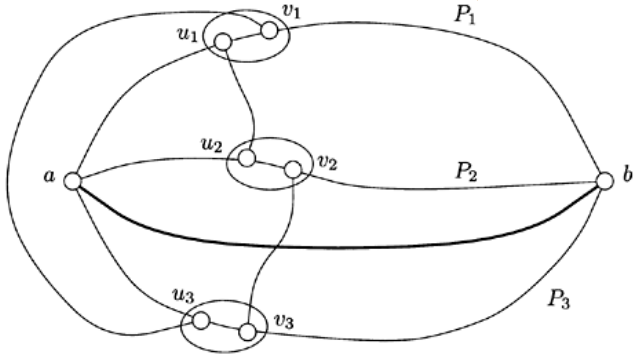
\includegraphics[scale=0.6]{img/minoreTK5.PNG}
                \caption{minore \(TK_5\) di \(G\)}
            \end{figure}
        \end{enumerate}
    \end{proof}
\end{teorema}
Il teorema di Kuratowski può essere riformulato in termini di minori, in questo caso esso prende il nome di teorema di Wagner.
\begin{teorema}[Teorema di Wagner]
    Un grafo \(G\) è planare se e solo se non ha \(K_{3,3}\) o \(K_5\) come minori.
    \begin{proof}
        \underline{“\(\Rightarrow\)”}: se \(G\) planare ovviamente non ha come minori \(K_{3,3}\) o \(K_5\). \\
        \underline{“\(\Leftarrow\)”}: se \(G\) non ha \(K_{3,3}\) o \(K_5\) come minori allora non ha nemmeno sottografi \(TK_{3,3}\) o \(TK_5\) e quindi è planare per il teorema di Kuratowski \(\ref{Kuratowski}\).
    \end{proof}
\end{teorema}
\chapter{L'algoritmo di Boyer-Myrvold}
% fare introduzione
\section{Supposizioni sul grafo in input}
% connesso
% numero archi-vertici
% biconnessso


% left-right planarity test or de Fraysseix–Rosenstiehl planarity criterion



\endgroup

%\titleformat{\chapter}
%{\normalfont\bfseries}{Allegato \thechapter}{1em}{#1}
% sezione Allegati - opzionale
\addto\captionsitalian{\renewcommand{\chaptername}{Allegato}}

\appendix
\chapter{Teoria dei grafi}
\begin{definizione}[Grafo]
    Un grafo è una coppia \(G=(V,E)\) dove:
    \begin{itemize}
        \item \(V\) è un insieme di vertici (\textbf{vertex});
        \item \(E\) è un insieme di coppie di nodi \((u,v),\;u,v\in V\) dette archi o lati (\textbf{edge});
    \end{itemize}
    Nei grafi \textbf{orientati} le coppie in \(E\) sono ordinate in quelli non orientati no.
\end{definizione}

\begin{definizione}[Adiacenza]
    Un vertice \(v\) si dice adiacente a \(u\) se esiste \((u,v) \in E\). \\
    NB:\@ nei grafi non orientati l'adiacenza è una relazione simmetrica.
\end{definizione}

\begin{definizione}[Arco incidente]
    Un arco \((u,v)\) si dice incidente da \(u\) a \(v\).
\end{definizione}

\begin{definizione}[Grado]
    Nel caso di grafi orientati definiamo:
    \begin{itemize}
        \item \textbf{grado entrante} di un nodo come il numero di archi incidenti su esso;
        \item \textbf{grado uscente} di un nodo come il numero di archi incidenti da esso.
    \end{itemize}
    Per i grafi non orientati avremo invece un'unica definizione:
    \begin{itemize}
        \item il \textbf{grado} di un nodo è il numero di archi incidenti su di esso.
    \end{itemize}
\end{definizione}

\begin{definizione}[Cammino]
    Sia \(G=(V,E)\) un grafo. Un cammino \(C\) di lunghezza \(k\) è una sequenza di nodi \(u_0,u_1 \dots, u_k\) t.c.
    \begin{equation}
        (u_i,u_{i+1})\in E \text{ per } 0 \leq i \leq k-1
    \end{equation}
\end{definizione}

\begin{definizione}[Grafi isomorfi]
    Siano \(G=(V(G),E(G)), H=(V(H),E(H))\) due grafi. Diremo \(G\) isomorfo a \(H\) se \(\exists \theta : V(G) \to V(H)\) t.c. \(\theta\) è un isomorfismo e
    \begin{equation}
        \theta(E(G)) \doteq \{ \theta(uv) \; t.c.\; uv \in E(G)\} = E(H)
    \end{equation}
\end{definizione}

\begin{definizione}[Grafo completo]
    Un grafo \(G=(V,E)\) si dice completo se
    \begin{equation}
        \forall u,v \in V \; \exists (u,v) \in E
    \end{equation}
    Definiamo \(K_n\) un grafo completo con \(n\) vertici.
\end{definizione}

\begin{definizione}[Grafo bipartito]
    Un grafo non orientato \(G=(V,E)\) si dice bipartito se \(V\) può essere diviso in due sottoinsiemi \(X,Y\) t.c.
    \begin{equation}
        \forall (u,v) \in E \text{ vale } u\in X,\; v\in Y \text{ oppure } u\in Y,\; v\in X
    \end{equation}
    Un grafo bipartito può avere al più \(|X|\cdot |Y|\) archi. \\
    Definaiamo inoltre \(K_{m,n}\) il grafo bipartito completo che soddisfa
    \begin{equation}
        |X|=m,\; |Y|=n,\; \varepsilon \doteq |E| = mn
    \end{equation}
\end{definizione}

\begin{definizione}[Connessione]
    Un grafo non orientato \(G=(V,E)\) è detto \textbf{connesso} se
    \begin{equation}
        \forall u,v \in V \; \exists (u,v) \in E
    \end{equation}
    Un sottografo connesso massimale di un grafo non orientato è detto \textbf{componente connessa}.
\end{definizione}

\begin{definizione}[Vertex-connectivity]
    Sia \(G=(V,E)\) un grafo non orientato. Definiamo \textbf{vertex-connectivity}  \(\kappa\) il minimo numero di vertici da eliminare per sconnettere \(G\).
\end{definizione}

\begin{definizione}[Grafo k-connesso]
    Sia \(G=(V,E)\) un grafo non orientato. Diremo \(G\) \textbf{k-connesso} se \(|V|>k\) e \(\kappa \geq k\) dove \(\kappa\) corrisponde alla vertex-connectivity.\\
    Informalmente un grafo è detto k-connesso se rimane connesso rimuovendo \(k'<k\) vertici qualsiasi.
\end{definizione}

\begin{teorema}[Grafo 2-connesso (Non separabile)]
    Un grafo non orientato \(G=(V,E),\; |V| \geq 3\) è 2-connesso \(\Leftrightarrow\) ogni coppia di vertici \((u,v)\) è connessa da almeno 2 cammini internamente disgiunti.
\end{teorema}

\begin{definizione}[Cut vertex]
    Vertoci che se eliminati sconnettono il grafo.
\end{definizione}

\begin{definizione}[Blocco]
    Definiamo blocchi di un grafo i sottografi 2-connessi massimali.
\end{definizione}

\begin{definizione}[Cammini internamente disgiunti]
    Sia \(G=(V,E)\) un grafo non orientato, siano \(a,b \in V\) due cammini da \(a\) a \(b\) \(a,v_1,\dots,v_n,b\), \(a,u_1,\dots,u_n,b\). Essi si dicono internamente disgiunti se
    \begin{equation}
        v_i \neq u_j\; \forall i,j
    \end{equation}
\end{definizione}

\begin{definizione}[Ciclo di Hamilton]
    Sia \(G=(V,E)\) un grafo non orientato. Definiamo ciclo di Hamilton un ciclo che contiene tutti i vertici del grafo una sola volta.\\
    Definiamo \(G\) hamiltoniano se \(G\) contiene un ciclo di hamilton.
\end{definizione}
% teo

\begin{definizione}[Suddivisione]
    Dato un grafo \(G\) definiamo suddivisione (subdivision) di \(G\) i grafi ottenuti da \(G\) rimpiazzando uno o più archi con cammini di lunghezza 2 o più. In altre parole una suddivisione di \(G\) è un grafo ottenuto da esso inserendo dei vertici “all'interno dei lati”.
\end{definizione}
\begin{figure}[H]
    \centering
    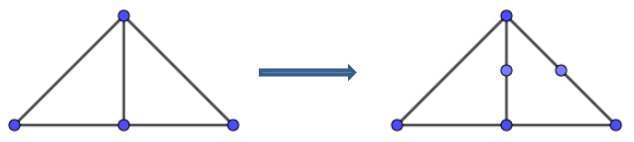
\includegraphics[scale=0.6]{img/suddivisione.PNG}
    \caption{esempio suddivisione}
\end{figure}
\begin{definizione}[Contrazione]
    Operazione inversa della suddivisione, consiste nell'contrarre un arco avente un endpoint di grado 2.
\end{definizione}

\begin{definizione}[Grafi omeomorfi]
    Due grafi \(G_1,G_2\) si dicono topologicamente equivalenti o omeomorfi se possono essere trasformati l'uno nell'altro attraverso operazioni di suddivisione o contrazione degli archi.
    \\ Denotiamo l'insieme dei grafi omeomorfi a \(G\) con \(TG\).
\end{definizione}

\begin{definizione}[Minore]
    \(H\) è detto minore di \(G\) se \(H\) è un grafo ottenuto da \(G\) tramite una sequenza di operazioni di rimozione di archi, vertici o contrazione di archi.
\end{definizione}

\begin{definizione}[Immersione planare]
    Dato un grafo \(G\), definiamo \(\psi : (V,E) \to \mathbb{R}^2\) la funzione che mappa i vertici di \(G\) nel piano e gli archi in curve continue che si intersecano solamente negli endpoint. Allora \(G^\psi \doteq \psi(G)\) è chiamata immersione planare di \(G\).
\end{definizione}

\begin{definizione}[Faccia]
    Le faccie di un immersione planare \(G^\psi\) sono le regioni connesse che rimangono quando il piano viene “tagliato” dagli archi di \(G^\psi\)
\end{definizione}

\begin{definizione}[Facial walk]
    Sia \(G\) grafo, \(G^\psi\) una sua immersione nel piano. Un cammino chiuso \(C\) frontiera di una faccia \(F\) di \(G^\psi\) è detto facial walk di F.
\end{definizione}

\begin{definizione}[Grado di una faccia]
    Definaiamo \(\deg(F)\) grado di una faccia \(F\) come la lunghezza del suo facial walk.
\end{definizione}
\begin{definizione}[Grafo semplice]
    Grafo contentente un numero finito di nodi.
\end{definizione}
\begin{definizione}[Grafo planare]
    Un grafo non orientato \(G\) si dice planare se può essere rappresentato nel piano evitando che gli archi si intersechino (se non negli endpoint).
\end{definizione}
\chapter{Topologia}
\begin{definizione}[n-cella chiusa]
    Spazio topologico omeomorfo ad una palla chiusa n-dimensionale.
\end{definizione}
\begin{definizione}[Complesso cellulare (CW-complesso)]
    Spazio topologico ottenuto incollando tra loro un insieme di celle chiuse.
\end{definizione}
\begin{definizione}[Caratteristica di eulero]\label{caratteristica-eulero}
    Sia \(\tau \subset \mathbb{R}^n\) un complesso cellulare composto da \(k_i\) i-celle \(i=0,\dots,n\). Definiamo caratteristica di eulero
    \begin{equation}
        \chi(\tau) = k_0 - k_1 + k_2 - \dots k_n = \sum_{i=0}^{n}{(-1)}^i k_i
    \end{equation}
\end{definizione}

\begin{definizione}[Cammini omotopi]
    Siano \(f,g \in \mathcal{C}^0(X;Y)\). Diciamo \(f\) e \(g\) omotope \(f \sim g\) se esiste \(H : X \times [0,1] \to Y\) t.c.
    \begin{equation}
        \forall x \in X \begin{cases}
            H(x,0)=f(x) \\
            H(x,1)=g(x)
        \end{cases}
    \end{equation}
    Informalmente questo vale se una mappa può essere “deformata con continutià” nell'altra.
\end{definizione}

\begin{definizione}[Spazi omotopicamente equivalenti]
    \(X,Y\) si dicono omotopicamente equivalenti (\(X\sim Y\)) se \(\exists f : X \to Y, g:Y \to X \) t.c.
    \begin{itemize}
        \item \(g \circ f \sim id_X\)
        \item \(f \circ g \sim id_Y\)
    \end{itemize}
    Informalmente \(X,Y\) saraano omotopicamente equivalenti se possono essere trasformati l'uno nell'altro con operazioni di deformazione.
\end{definizione}

\begin{lemma}[Omotopicamente invariante]\label{om-inv}
    La caratteristica di eulero è un omotopicamente invariante, ovvero
    \begin{equation}
        X \sim Y \Rightarrow \chi (X) = \chi (Y)
    \end{equation}
\end{lemma}

\begin{proposizione}[Invarianza topologica]\label{inv-top}
    La caratteristica di eulero è un invariante topologico, ovvero
    \begin{equation}
        X \simeq Y \Rightarrow \chi (X) = \chi (Y)
    \end{equation}
    dove \(X \simeq Y\) se \(X\) e \(Y\) omeomorfi.
\end{proposizione}

\begin{lemma}
    Ogni poliedro semplice può essere identificato come un grafo planare usando i vertici del poliedro come vertici del grafo e gli spigoli del poliedro come archi del grafo.
\end{lemma}
\begin{proposizione}
    Sia \(\tau\) un poliedro semplice allora \(\chi(\tau)=2\)
    \begin{proof}
        Questo risultato segue direttamente dal lemma precedente e dal corollario \(\ref{formulaeulero}\).
    \end{proof}
\end{proposizione}

% bibliografia in formato bibtex
%
% aggiunta del capitolo nell'indice
\addcontentsline{toc}{chapter}{Bibliografia}
% stile con ordinamento alfabetico in funzione degli autori
\bibliographystyle{plain}
\nocite{*}\bibliography{biblio}
%%%%%%%%%%%%%%%%%%%%%%%%%%%%%%%%%%%%%%%%%%%%%%%%%%%%%%%%%%%%%%%%%%%%%%%%%%
%%%%%%%%%%%%%%%%%%%%%%%%%%%%%%%%%%%%%%%%%%%%%%%%%%%%%%%%%%%%%%%%%%%%%%%%%%
%% Nota
%%%%%%%%%%%%%%%%%%%%%%%%%%%%%%%%%%%%%%%%%%%%%%%%%%%%%%%%%%%%%%%%%%%%%%%%%%
%% Nella bibliografia devono essere riportati tutte le fonti consultate 
%% per lo svolgimento della tesi. La bibliografia deve essere redatta 
%% in ordine alfabetico sul cognome del primo autore. 
%% 
%% La forma della citazione bibliografica va inserita secondo la fonte utilizzata:
%% 
%% LIBRI
%% Cognome e iniziale del nome autore/autori, la data di edizione, titolo, casa editrice, eventuale numero dell’edizione. 
%% 
%% ARTICOLI DI RIVISTA
%% Cognome e iniziale del nome autore/autori, titolo articolo, titolo rivista, volume, numero, numero di pagine.
%% 
%% ARTICOLI DI CONFERENZA
%% Cognome e iniziale del nome autore/autori (anno), titolo articolo, titolo conferenza, luogo della conferenza (città e paese), date della conferenza, numero di pagine. 
%% 
%% SITOGRAFIA
%% La sitografia contiene un elenco di indirizzi Web consultati e disposti in ordine alfabetico. 
%% E’ necessario:
%%   Copiare la URL (l’indirizzo web) specifica della pagina consultata
%%   Se disponibile, indicare il cognome e nome dell’autore, il titolo ed eventuale sottotitolo del testo
%%   Se disponibile, inserire la data di ultima consultazione della risorsa (gg/mm/aaaa).    
%%%%%%%%%%%%%%%%%%%%%%%%%%%%%%%%%%%%%%%%%%%%%%%%%%%%%%%%%%%%%%%%%%%%%%%%%%
%%%%%%%%%%%%%%%%%%%%%%%%%%%%%%%%%%%%%%%%%%%%%%%%%%%%%%%%%%%%%%%%%%%%%%%%%%
\end{document}
